% Adapted from the VGTC template for the Data Visualization Interim Report

\documentclass{vgtc}                          % final/conference style
%\documentclass[review]{vgtc}                 % review
%\documentclass[widereview]{vgtc}             % wide-spaced review
%\documentclass[preprint]{vgtc}               % preprint
%\documentclass[electronic]{vgtc}             % electronic version

\ifpdf
  \pdfoutput=1\relax
  \pdfcompresslevel=9
  \pdfoptionpdfminorversion=7
  \ExecuteOptions{pdftex}
  \usepackage{graphicx}
  \DeclareGraphicsExtensions{.pdf,.png,.jpg,.jpeg}
\else
  \ExecuteOptions{dvips}
  \usepackage{graphicx}
  \DeclareGraphicsExtensions{.eps}
\fi

\graphicspath{{figures/}{pictures/}{images/}{./}}

\usepackage{microtype}
\PassOptionsToPackage{warn}{textcomp}
\usepackage{textcomp}
\usepackage{mathptmx}
\usepackage{times}
\renewcommand*\ttdefault{txtt}
\usepackage{cite}
\usepackage{booktabs}
\usepackage{array}

\onlineid{0}
\vgtccategory{Research}
\vgtcinsertpkg

\title{Data Visualization Interim Report}

\author{S.P. Verbeek (2010498)\and P.C. Villadangos (2108602)}

\abstract{This interim report presents the design rationale for an interactive visualization dashboard, \emph{Tourism Structural Explorer}. The dashboard supports exploratory analysis of how tourism dependence relates to employment composition and selected development indicators across countries and years. Rather than claiming causal effects, the project focuses on comparative analysis, outlier detection, country-specific temporal pathways, and awareness of data coverage limitations.}

\CCScatlist{
  \CCScatTwelve{Human-centered computing}{Visualization}{Visualization application domains}{};
  \CCScatTwelve{Human-centered computing}{Visualization}{Visualization systems and tools}{}
}

% Assignment/report version: remove conference copyright block.
\nocopyrightspace

\begin{document}

\firstsection{Introduction}
\maketitle

Tourism is frequently discussed as a possible development pathway for countries that rely on international visitors, foreign exchange, and service-sector employment. However, the relationship between tourism dependence and a larger structural transformation is not straightforward. A country with high tourism revenues may show a more service-oriented employment structure, but may also differ in GDP per capita, urbanization, poverty, and inequality. Therefore, the goal of this project is not to prove causal effects of tourism, but to support exploratory comparison of country-level patterns over time.

We design an interactive visualization dashboard for development-oriented analysts, students, and policy researchers who want to explore how tourism dependence relates to employment composition and selected development outcomes. The main goal of the domain is to help users compare countries, identify outliers, and follow country-specific development over time.

Visualization is appropriate for this problem because the relevant questions are open-ended and comparative, making human-centered exploratory analysis more suitable than fully automated approaches~\cite{munzner2014}. A single statistic, such as a correlation coefficient, cannot show whether countries follow different structural pathways, whether regional groups behave differently, or whether observed patterns are affected by missing values.

\section{Data Analysis: What}

\subsection{Domain Data Specification}

The project uses World Development Indicators data~\cite{wdi}. The main domain variables are international tourism receipts as a percentage of total exports, which serves as an indicator of how much a country relies on tourism,  employment shares (male, female and, total) in services, industry, and agriculture, GDP per capita, urban population share, poverty headcount, and the Gini index. The dashboard explores tourism receipts and their relation with employment share composition, GDP per capita, urbanization, poverty, inequality, country pathways over time, and cross-country comparisons. 

Several conceptual data issues influence the design. First, World Development Indicators are not always available for every country and year. The dashboard therefore distinguishes exact-year values from the latest available values up to a selected year. Second, some variables are derived from multiple original indicators: for example, male and female employment shares are averaged into sector-level employment indicators. Third, missingness is not treated only as a preprocessing inconvenience; it is visualized through a data coverage matrix so that users can judge whether a comparison is reliable.

\subsection{Data Abstraction}

At the abstract level, the dataset is a static multidimensional table. Each observation is indexed by the composite key \emph{country} $\times$ \emph{year}; the remaining attributes are measured or derived values. The main items are therefore country--year observations, while countries are also used as higher-level items when comparing trajectories, structural shifts, and data coverage. Although the data is country-based, geographic position is not part of the current abstraction. Countries are treated as categorical items instead of spatial objects. The main attributes, their roles, and their abstract types are summarized in~\autoref{tab:data-abstraction}.

\begin{table*}[t]
    \centering
    \caption{Data abstraction of the main attributes used in the dashboard.}
    \label{tab:data-abstraction}
    \footnotesize
    \setlength{\tabcolsep}{4pt}
    \renewcommand{\arraystretch}{1.12}
    \begin{tabular}{p{0.27\textwidth} p{0.30\textwidth} p{0.35\textwidth}}
        \toprule
        \textbf{Attribute} & \textbf{Role} & \textbf{Abstract type} \\
        \midrule

        Country &
        Item identifier; part of the composite key &
        Categorical key \\

        Year &
        Temporal index; part of the composite key &
        Ordered quantitative key; sequential \\

        Region &
        Grouping attribute &
        Categorical \\

        International tourism receipts as \% of exports &
        Main explanatory value attribute for tourism dependence &
        Quantitative sequential value \\

        Employment in services, industry, and agriculture &
        Main outcome values; three-sector employment composition &
        Quantitative sequential values; constrained part-to-whole composition \\

        Employment group: total, male, female &
        Selector for different employment variants &
        Categorical \\

        Development indicators: GDP per capita, urban population share, poverty headcount, Gini index &
        Outcome value attributes used to compare broader development patterns &
        Quantitative sequential values \\

        Exact-year value vs. latest available value &
        Derived data-status attribute indicating how a value was obtained &
        Categorical \\

        Data coverage per country and indicator &
        Derived reliability attribute for missingness inspection &
        Quantitative sequential value, or ordinal if binned \\

        Structural employment shift &
        Derived change attribute: latest available share minus first available share &
        Quantitative diverging value \\

        \bottomrule
    \end{tabular}
\end{table*}


\section{Task Analysis: Why}

\subsection{Domain-Specific Tasks}

The intended users need to perform exploratory comparisons across countries and years. The task analysis is organized from high-level goals to lower-level analytical tasks, because the dashboard is intended for open-ended exploration rather than presentation of a known conclusion.

\textbf{High-level goal.}
Users should be able to generate and inspect hypotheses about whether tourism-dependent countries show more service-oriented employment structures, and whether these patterns relate to broader development outcomes over time. The goal is not to prove causality, but to support exploratory reasoning about patterns, exceptions, and country-specific pathways.

\textbf{Mid-level domain tasks.}
The high-level goal is decomposed into the following domain tasks:

\begin{itemize}
    \setlength\itemsep{0pt}
    \item \textbf{T1:} Assess whether countries with higher tourism dependence tend to have a more service-oriented employment structure.
    \item \textbf{T2:} Compare how tourism dependence relates to GDP per capita, urbanization, poverty, and inequality.
    \item \textbf{T3:} Compare whether countries from different regions show different tourism--employment or tourism--development patterns.
    \item \textbf{T4:} Follow one country's employment composition over time to inspect its structural pathway.
    \item \textbf{T5:} Compare how employment shares changed from the first available year to the latest available year across countries and sectors.
    \item \textbf{T6:} Check whether missing or substituted values affect the reliability of a comparison.
\end{itemize}

\textbf{Low-level analytical tasks.}
To carry out these domain tasks, users need to compare country-year values, identify outliers and extrema, summarize groups of countries, follow one country's ordered sequence of years, inspect first-to-latest changes, and check whether observed patterns are supported by sufficient data coverage.

\subsection{Task Abstraction}

The domain tasks are translated into Munzner-style action--target pairs~\cite{munzner2014}  in~\autoref{tab:task-abstraction}. The abstraction deliberately removes domain-specific terms such as tourism, employment, and poverty: it describes what analytical operation is performed and what type of data pattern is sought.

\begin{table}[t]
    \centering
    \caption{Task abstraction derived from the domain-specific tasks.}
    \label{tab:task-abstraction}
    \footnotesize
    \setlength{\tabcolsep}{3pt}
    \renewcommand{\arraystretch}{1.12}
    \begin{tabular}{@{}p{0.12\linewidth} p{0.33\linewidth} p{0.45\linewidth}@{}}
        \toprule
        \textbf{Task} & \textbf{Abstract action} & \textbf{Abstract target} \\
        \midrule

        T1 &
        Discover; Compare &
        Correlation between quantitative attributes; outliers \\

        T2 &
        Discover; Compare; Summarize &
        Correlation and distribution across multiple quantitative attributes \\

        T3 &
        Compare; Summarize &
        Distribution and clusters across categorical groups \\

        T4 &
        Identify; Summarize &
        Trend of one item over ordered time \\

        T5 &
        Compare &
        Trends and extrema across items and attributes \\

        T6 &
        Summarize; Identify &
        Feature: data availability and missingness patterns \\

        \bottomrule
    \end{tabular}
\end{table}

These abstractions guide the later design choices. T1--T3 require views that support comparison of quantitative relationships and group patterns. T4 requires a representation of ordered temporal change. T5 requires a compact comparison of change magnitudes across countries and sectors. T6 requires an explicit overview of data availability so that users can judge whether a visible pattern is reliable.

\section{Current Solution: Tourism Structural Explorer}

The current solution is an interactive Dash dashboard named \emph{Tourism Structural Explorer}. The tool uses coordinated multiple views to support overview, filtering, comparison, and country analysis. Its purpose is to help users explore whether tourism dependence is associated with structural changes in employment and with broader development outcomes. The design follows the “What, Why, How” visualization framework and nested model discussed by Munzner~\cite{munzner2014}. The design is directly derived from the task abstraction in~\autoref{tab:task-abstraction}: the association views address T1--T3, the country trajectory view addresses T4, the structural shift view addresses T5, and the data coverage matrix addresses T6.

\begin{figure}[t]
    \centering
    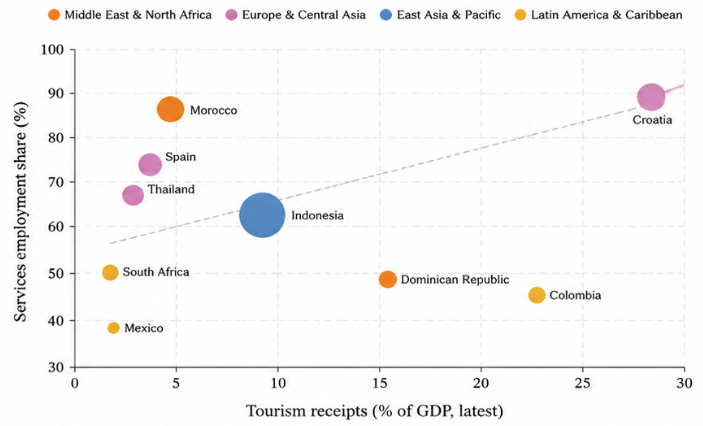
\includegraphics[width=\linewidth]{graphgraph.png}
    \caption{Compares tourism dependence with service employment-sector share, the point position encodes quantitative values and color hue encodes region.}
    \label{fig:scatterplot-view}
\end{figure}

\begin{figure}[t]
    \centering
    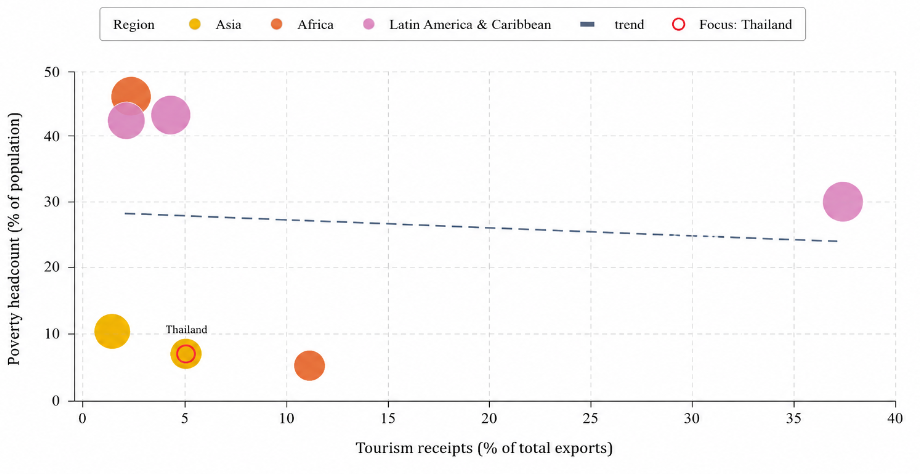
\includegraphics[width=\linewidth]{graphgraph3.png}
    \caption{Compares tourism dependence with poverty headcount ratio, the point position encodes quantitative values and color hue encodes region.}
    \label{fig:scatterplot2-view}
\end{figure}

The dashboard includes global controls for selected countries, focus country, comparison year, data mode, employment sector, and development outcome. These controls allow users to adjust the scope of the analysis and dynamically change which variables are encoded in the visualizations. This makes the tool flexible enough to support both broad cross-country exploration and more focused country-level inspection.

Alternative designs were considered but rejected for task-fit reasons. \\
A choropleth map was not used because the main tasks involve comparing country attributes and trajectories instead of analyzing geographic adjacency. Separate line charts could show sector changes over time, but they would not directly encode the three-part employment composition. Grouped or stacked bar charts were also less suitable for the structural shift view because they make multi-sector change comparison more cluttered than a shared-axis dotplot.

\subsection{Association Views}

In the dashboard, right below the controls, the first two graphs shown are scatterplots. The first scatterplot as seen in~\autoref{fig:scatterplot-view} compares international tourism receipts with a selected employment-sector variable, such as employment in services, industry, or agriculture. Users can select total, male, or female employment percentages. The second scatterplot, as seen in~\autoref{fig:scatterplot2-view} compares tourism receipts with a selected development outcome, such as GDP per capita, poverty headcount, or the Gini index.

In both views, each mark represents a country. Horizontal and vertical position encode quantitative variables, which is appropriate because aligned spatial position is one of the most effective visual channels for comparing numerical values according to Munzner’s ranking of visual channels~\cite{munzner2014}. Region is encoded using color hue, since it is a categorical attribute. Marker size is used only as secondary contextual information, such as GDP per capita in the left employment graphic or service employment share in the right development indicator graphic, because area is less precise than position for quantitative judgment.

These scatterplots support the tasks of discovering associations, identifying outliers, and comparing countries. To help users interpret the overall association, a dashed trend line summarizes the relationship for the selected countries. The trend line is used only as an exploratory visual summary: the observed relationships represent correlations and associations, not causal effects.


\subsection{Composition and Pathway Views}

A ternary plot is used to represent the employment structure of each country because agriculture, industry, and services form a three-part compositional relationship. Each point in the plot represents one country-year observation, and its position is determined by the relative share of employment in the three sectors. The ternary plot allows users to interpret the relative employment composition of a country. Each point is positioned according to the share of employment in agriculture, industry, and services, which together form a three-part composition. The gridlines provide approximate values, while exact sector percentages are available through hover interaction. Therefore, the ternary view is mainly used to identify compositional patterns and directional change rather than to read precise numerical values.

This representation is suitable for the project because the main analytical objective is to examine structural transformation rather than changes in a single sector independently. Although a standard line chart can show the evolution of each sector separately, it does not directly represent the balance between the three sectors as a compositional structure~\cite{munzner2014}. In contrast, the ternary plot allows users to interpret employment structure as a whole and to observe whether a country’s economy moves toward a more service-oriented, industry-oriented, or agriculture-oriented composition.

\begin{figure}[t]
    \centering
    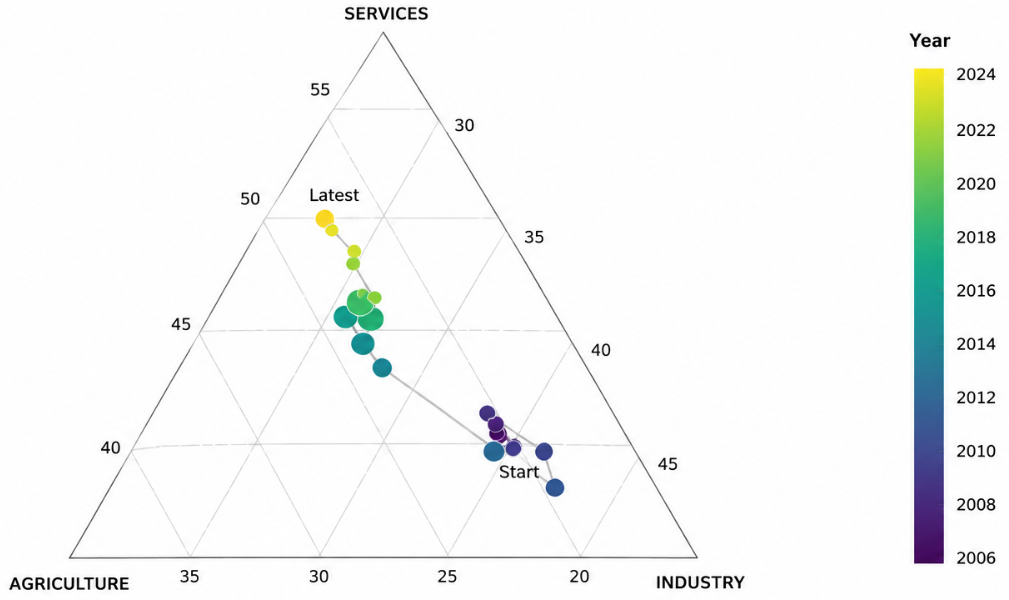
\includegraphics[width=\linewidth]{ternaryview2.png}
    \caption{Share in employment sectors over time for Thailand. Each point represents a year observation, and the connecting line shows how employment shifts between employment-sectors.}
    \label{fig:ternary-view}
\end{figure}

The dashboard includes two ternary views. The first shows the employment composition of the selected countries for the chosen comparison year, supporting cross-country comparison within the same compositional space. ~\autoref{fig:ternary-view} shows the trajectory of a selected focus country over time. In this trajectory view, each point represents a year, and the connecting line shows the direction of structural change. 

The ternary view also supports the central hypothesis of the project by making service-sector specialization visually observable. If countries with higher tourism dependence appear closer to the services vertex, or move toward it over time, this may suggest an association between tourism dependence and service-oriented structural transformation. However, the visualization is used for exploratory analysis only and does not establish a causal relationship between tourism and changes in employment structure.

One limitation of ternary plots is that they are less familiar than standard Cartesian charts and are less effective for precise numerical reading. For this reason, the dashboard uses the ternary plot primarily to support pattern recognition, comparison, and interpretation of directional change. Exact sector values are provided through hover interaction, allowing users to access detailed information on demand.

\subsection{Structural Shift and Data Coverage}

The structural shift view summarizes how the employment structure of each selected country changed between the earliest and most recent available observations. Instead of showing the entire time series, the visualization focuses on the overall change in employment shares across agriculture, industry, and services. Changes are represented in percentage points, which makes it possible to compare both the direction and the scale of sectoral change across countries.

This view is displayed as a dotplot using a shared horizontal axis. Values located to the right of zero indicate that the employment share of a sector increased over time, while values to the left indicate a decline. A dotplot was chosen because it allows changes across multiple countries and sectors to be compared clearly without the clutter that can appear in grouped or stacked bar charts. Different colors and marker shapes are used to distinguish the three sectors and improve readability.

\begin{figure}[t]
    \centering
    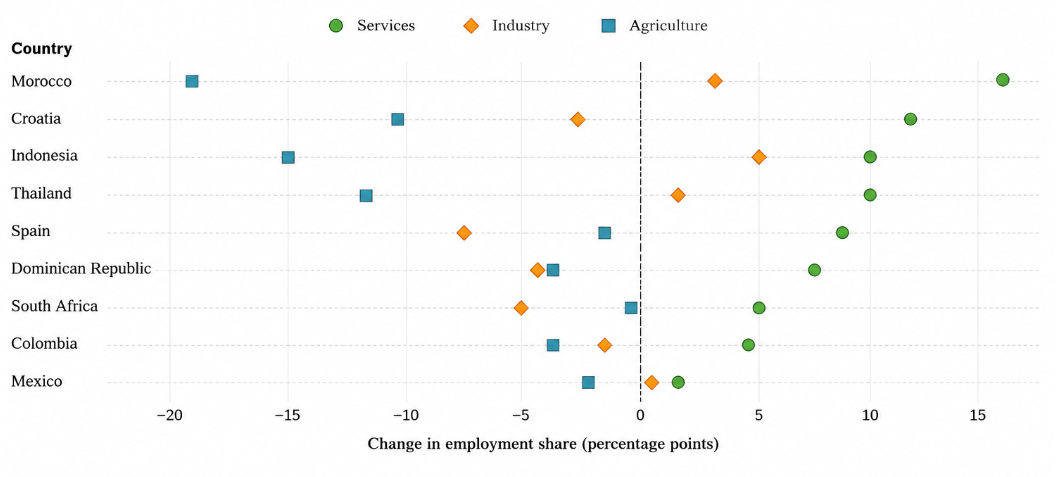
\includegraphics[width=\linewidth]{shiftview.png}
    \caption{Structural employment shift by country and sector. Each mark shows the percentage-point change between the earliest and latest available observations.}
    \label{fig:shift-view}
\end{figure}

The structural shift view complements the ternary trajectory visualization. The ternary plot helps illustrate how the balance between sectors evolves over time, whereas the dotplot provides a more direct summary of the magnitude of change. Used together, the two views support both the interpretation of broader structural patterns and the comparison of specific sectoral shifts.

The dashboard also includes a data coverage matrix that makes missing values visible. Countries and indicators are arranged in a grid, and color intensity represents the proportion of available observations. This is particularly relevant because several indicators in the World Development Indicators dataset, especially tourism, poverty, and inequality measures, are not consistently available across countries and years.

Rather than hiding incomplete data or removing missing observations without explanation, the dashboard exposes differences in coverage directly in the interface. This helps users evaluate how reliable a comparison is before interpreting the results. For instance, employment-sector indicators are available for most countries over long time periods, while poverty and inequality variables are often more fragmented. Showing data availability explicitly therefore improves transparency and helps contextualize the patterns displayed in the other visualizations.



\subsection{Interaction and Coordinated Views}

The main interaction strategy follows Shneiderman’s information-seeking mantra~\cite{shneiderman1996}: overview first, zoom and filter, then details on demand. Users first obtain an overview through the scatterplots and composition views. They can then filter by country, region, year, sector, and outcome variable. Finally, they can inspect detailed values through hover interaction or by selecting a focus country.

Clicking a country in the first scatterplot updates the focus country, which in turn changes the country trajectory view. This creates a coordinated multiple-view interaction in which a selection in one view determines the detailed representation shown in another. This interaction supports the transition from global pattern detection to country-level analysis.

Using Yi et al.’s interaction vocabulary~\cite{yi2007}, the dashboard supports several interaction types. Filter is supported through country and year controls. Encode is supported through dropdown menus that allow users to change the selected employment or development variable. Select is implemented through click-to-focus interaction. Connect is achieved through linked updates between the scatterplots and the focus-country trajectory. Finally, Abstract/Elaborate is supported by combining overview scatterplots with detailed country trajectories, structural shift summaries, and hover tooltips.

Overall, the current solution is designed as an exploratory visual analysis tool. It does not attempt to prove that tourism causes structural transformation. Instead, it helps users compare countries, detect patterns, inspect temporal pathways, and generate hypotheses about how tourism dependence relates to employment structure and development outcomes.

\section{Implementation}

The dashboard is implemented in Python using Dash~\cite{dash}, Plotly~\cite{plotly}, pandas~\cite{pandas}, and NumPy~\cite{numpy}. The main application file is \texttt{tourism\_structural\_dashboard\_designed.py}. The repository also contains the two CSV data files, a standard \texttt{requirements.txt}, presentation notes, AI usage notes, and project guidance notes. The app is run locally with \texttt{python tourism\_structural\_dashboard\_designed.py} after installing the required packages.

\bibliographystyle{abbrv-doi}
\bibliography{references}
\end{document}
